\chapter{Systeemarchitectuur}
\label{ch:systeemarchitectuur}
\section{High-level systeem model}
Het project bestaat uit twee delen. Het eerste deel is de webapplicatie die gebruikt wordt door de actor. Het tweede deel is de MP4 Converter. Dit is een aparte module dat video's van allerlei formaten omvormt tot het standaardformaat dat gebruikt wordt in de applicatie, namelijk .mp4.
\subsection{Webapplicatie}
De webapplicatie wordt geprogrammeerd met gebruik van de MEAN \footnote{\url{http://mean.io/}} stack. Dit is een verzameling van technologieën die samen gebruikt worden om webapplicaties te ontwikkelen. De MEAN stack bevat volgende onderdelen:
\begin{itemize}
 \item \textbf{M}ongoDb: Dit is een open source NoSQL databank dat gebruik maakt van JSON documenten om gegevens te bewaren. 
 \item \textbf{E}xpress: Dit is een implementatie van Node dat geschikt is voor het opstellen van webservers. 
 \item \textbf{A}ngular: Dit is een client-side javascript framework dat geschikt is voor het creëren van dynamische webapplicaties. De interactie tussen het DOM en javascript wordt vereenvoudigt met Angular.
 \item \textbf{N}ode.js: Dit is een javascript runtime omgeving met als onderliggende basis de javascript engine van Chrome. Een gevolg van Node is het node packaging systeem (npm) dat toelaat om modules toe te voegen aan een applicatie met slechts één lijn code.
\end{itemize}
Hoe deze componenten met elkaar samenwerken kan bekeken worden op figuur \ref{fig:deploymentdiagram}.

\subsection{MP4 Converter}
De MP4 Converter is geprogrammeerd in Java en wordt gebruikt door de webapplicatie om videobestanden van verschillende formaten om te zetten naar het mp4 formaat. Als onderliggende basis wordt gebruik gemaakt van \texttt{ffmpeg} \footnote{\url{https://ffmpeg.org/}}. Dit is een handige tool dat toelaat om video's of geluid op te nemen en te converteren. Deze applicatie maakt enkel gebruik van het converteren van een video. De MP4 Converter is met andere woorden een Java wrapper voor ffmpeg met slechts beperkte functionaliteit.




\section{Klassendiagram}
\begin{figure}[ht]
	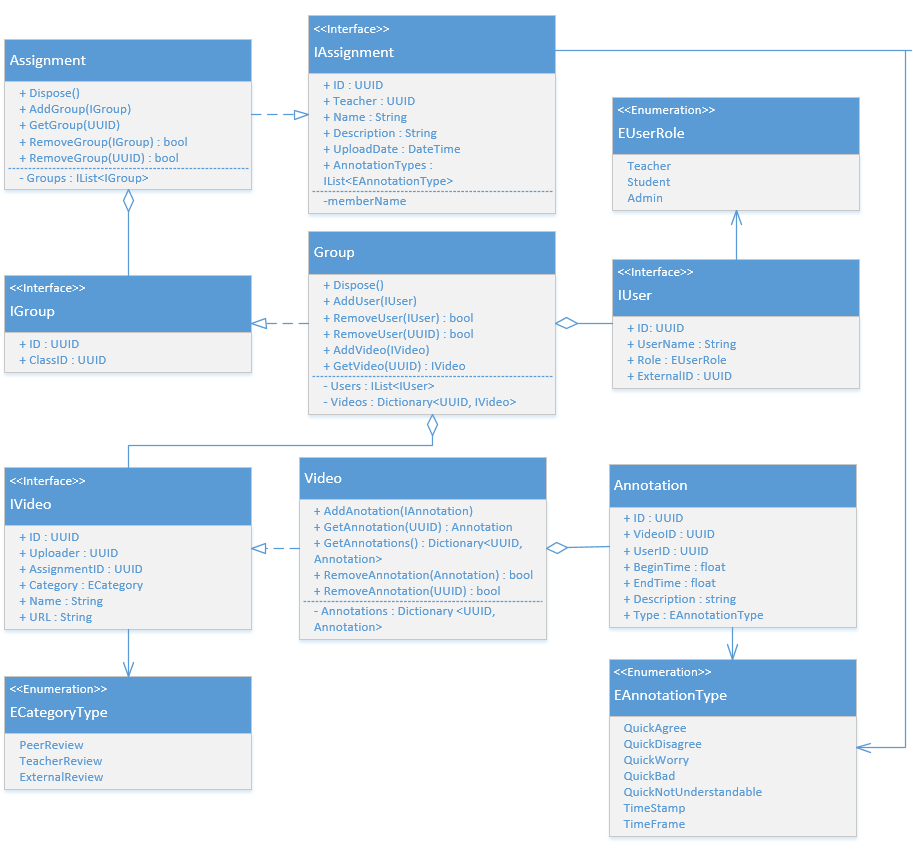
\includegraphics[width=\textwidth]{klassendiagram}
	\caption{Het klassendiagram}
	\label{fig:klassendiagram}
\end{figure}

In figuur \ref{fig:klassendiagram} is een overzicht te vinden van het klassendiagram. Dit diagram komt overeen met de implementaties van de verschillende database modelklassen en de manier hoe ze in relatie tot elkaar staan in de backend.
%% TODO: Informatie uitbreiden

\section{Deploymentdiagram}
\begin{figure}[ht]
	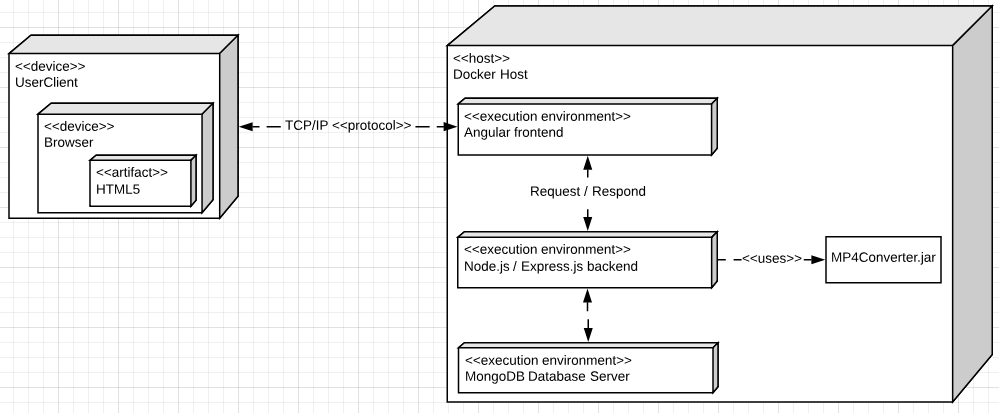
\includegraphics[width=\textwidth]{deploymentdiagram}
	\caption{Het deploymentdiagram}
	\label{fig:deploymentdiagram}
\end{figure}
In figuur \ref{fig:deploymentdiagram} is een overzicht te vinden van het deploymentdiagram. De applicatie draait in drie aparte docker containers op de server: de Node.js container (backend), de Angular frontend container en de MongoDB database container. 

\section{Databank}
De databank is opgesteld in MongoDB. Dit is een NoSQL omgeving waardoor het moeilijk is om een databankdiagram op te stellen. Om een overzicht te hebben van de relaties tussen de verschillende klassen zoals ze zijn ge\"implementeerd in de code kan gekeken worden naar het klassendiagram op figuur \ref{fig:klassendiagram}


\section{Sequentiediagrammen}

\begin{figure}
	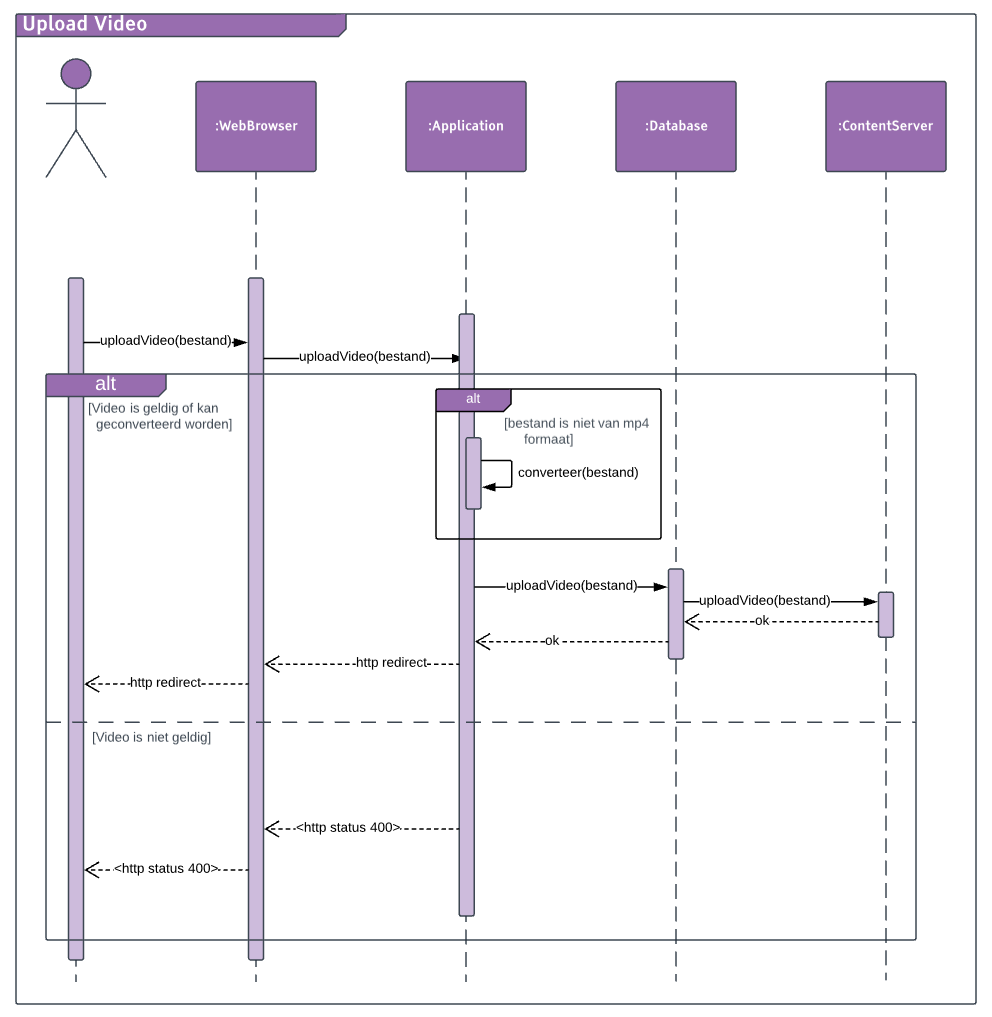
\includegraphics[width=\textwidth]{seq_diagram//SEQ_Upload_Video}
	\caption{Sequentiediagram van upload video}
	\label{fig:seq_upload_video}
\end{figure}

\begin{figure}
	\includegraphics[width=\textwidth]{seq_diagram//SEQ_plaats_annotatie}
	\caption{Sequentiediagram van show video}
	\label{fig:seq_show_video}
\end{figure}
Figuren \ref{fig:seq_upload_video} en \ref{fig:seq_show_video} zijn sequentiediagrammen van twee belangrijke events die kunnen voorkomen in de applicatie. De verschillende events maken gebruik van synchrone gebruikersinput die asynchroon wordt behandeld.
